\documentclass[12pt]{article}
% Preamble
\usepackage[left=2cm,top=2cm,right=2cm,nohead,nofoot]{geometry}
\usepackage{setspace}
\usepackage{graphicx}

% Header
\title{CS457 Assignment 1}
\author{Daniel Burstyn (20206120)}
\date{March 2, 2009}

% Body
\begin{document}
\maketitle
\tableofcontents
\doublespace
\newpage

\section{Pseudocode}
Below is a breif pseudocode description of my simulation code, modeled after
notes 5.

\subsection{State variables}
\begin{itemize}
\setlength{\itemsep}{-3mm}
\item $k$ - Item with ID k is to be transmitted next
\item $g$ - Keep track of when to handle i-requests (when $g = G$)
\item $nt$ - Number of users in the thinking state
\item request\_set - Contains t\_arrival (time of arival) and item ID of a
user's request for an f-item, and whether the the request is for an i-item or an
f-item
\item irequest\_queue - Contains t\_arrival of requests for i-items in a
queueing structure
\end{itemize}

\subsection{Event types}
\begin{itemize}
\setlength{\itemsep}{-3mm}
\item F-Arrival
\item I-Arrival
\item Departure (parameters:t\_arrival,type)
\item Start\_Transmit (paramters:k,g)
\item End\_Simulation
\end{itemize}

\subsection{Initialization}
\begin{itemize}
\setlength{\itemsep}{-3mm}
\item clock = 0
\item $nt$ = $N$
\item initialize event\_set to empty
\item initialize request\_set to empty
\item initialize irequest\_queue to empty
\item for $n = 1, 2, \dots, N$\\
\verb!    !determine think\_t\\
\verb!    !schedule an F-Arrival event at clock + think\_t\\
end for
\item k = 1
\item g = 1
\item determine interarrival\_t (interarrival time for i-request)
\item schedule a I-Arrival at clock + interarrival\_t
\item schedule a Start\_Transmit(k,g) event at clock
\item schedule an End\_Simulation event at time term\_sim
\end{itemize}

\subsection{F-Arrival event}
\begin{itemize}
\setlength{\itemsep}{-3mm}
\item nt = nt -1
\item determine id of item requested by user
\item enter entry (clock, id, f-item) to request\_set
\end{itemize}

\subsection{I-Arrival event}
\begin{itemize}
\setlength{\itemsep}{-3mm}
\item enter entry (clock, 0, i-item) to request\_set
\item determine interarrival\_t (interarrival time for i-request)
\item schedule a I-Arrival at clock + interarrival\_t
\end{itemize}

\subsection{Start\_Transmit event}
\begin{itemize}
\setlength{\itemsep}{-3mm}
\item determine transmit\_t, transmission time of an information item
\item If g = G then\\
\verb!    !g = 0\\
\verb!    !if irequest\_queue is non-empty then\\
\verb!        !remove entry from queue, and retrieve t\_arrival, and type\\
\verb!        !schedule a departure(t\_arrival, type) at clock + transmit\_t\\
\verb!    !end if\\
end if
\item else\\
\verb!    !for each entry in request\_set\\
\verb!        !if item\_id = k then\\
\verb!            !remove entry from set, and retrieve t\_arrival, and type\\
\verb!            !schedule a departure(t\_arrival, type) at clock +
transmit\_t\\
\verb!        !end if!\\
\verb!    !end for\\
k = k + 1\\
g = g + 1\\
if k $>$ N, then k = 1
\item schedule a Start\_Transmit(k,g) event at clock + transmit\_t
\end{itemize}

\subsection{Departure event}
\begin{itemize}
\setlength{\itemsep}{-3mm}
\item If type = f-item\\
\verb!    !record metrics\\
\verb!    !nt = nt + 1\\
\verb!    !determine think\_t\\
\verb!    !schedule an F-Arrival event at clock + think\_t
\item else\\
\verb!    !record metrics\\
end if
\end{itemize}

\subsection{End\_Simulation event}
\begin{itemize}
\setlength{\itemsep}{-3mm}
\item Exit main loop
\end{itemize}

\section{Part b) Length Of Run Determination}
\subsection{Analysis}
For this problem, I chose the values $L = 50000$ and $m = 8$ to generate my
confidence interval.  The results of these simulations can be found on the
following page.

From my 8 replications, I took the average of each of the $R$ values to get a
sample mean of $\approx 14.31$.  The standard deviation of the $R$ values was
also calculated to be $s \approx 0.063$.  The $t$ value is listed in the
textbook as 2.365 as $t_{(7, 0.975)}$ which is the value for a 95\% confidence
interval for 7 degrees of freedom.

The confidence interval was then computed using interval$ = 2 * t *
\frac{s}{\sqrt{m}} \approx 0.105$.  The $\pm 1\%$ inteval is simply $0.02 *
$sample mean $ \approx 0.286$.  We can see that our 95\% confidence interval is
will without the $\pm 1\%$ interval and we can conclude that the chosen $L$ of
50000 is a valid run length for our simulation in order to get sufficiently
accurate results.

\newpage
\begin{table}[htp!]
\subsection{Raw Data}
\begin{center}
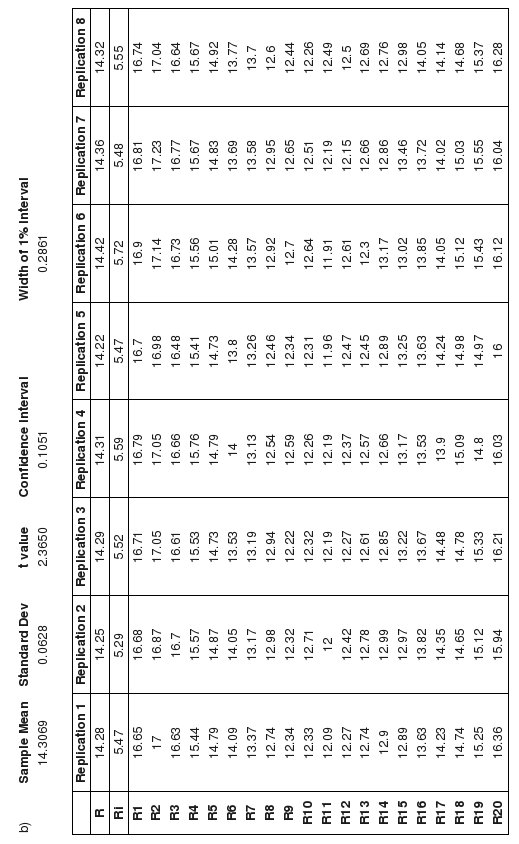
\includegraphics[height=20cm]{part_b.jpg}
\caption{Raw data for part b)}
\end{center}
\end{table}
\newpage

\section{Part c) Data Retrieved from Varying Factors}
The raw data is attached at the end of this report, and each graph will be
presented when it is discussed in part (d).

\section{Part d) Analysis of Varied Factors}

\begin{table}[htp!]
\subsection{Zipf vs Uniform Distributions}
\begin{center}
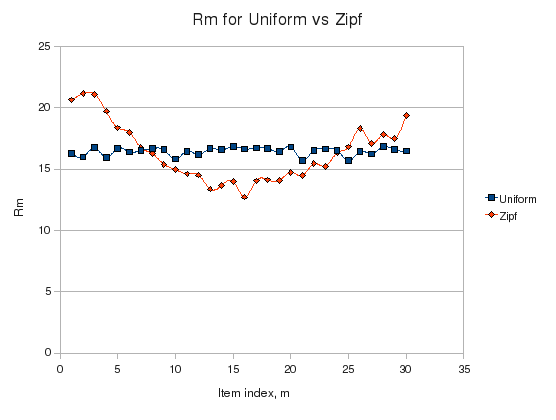
\includegraphics[height=10cm]{uniform_vs_zipf.png}
\end{center}
\end{table}

Looking at the graph above, we can see that uniform's $R_m$ values are all
approximatey the same.  This is to be expected since the items are both
requested with a uniform distribution (each item has the same likelihood of
being chosen) and each item is served for the same amount of time on average
since we serve them in a circular fashion for the same mean time.

We can also see that the zipf distribution is quite different from the uniform
distribution.  In particular, notice that both the low $R_m$s and the high
$R_m$s are higher than in the uniform distribution, and the middle range $m$
produce lower $R_m$s for the zipf distribution.

The formula for the zipf distribution indicates that the first item has a
particular probability of being chosen, $c$.  The second item has half that
chance of being picked, the third item one third of $c$, and so on.  This would
indicate that the lower id f-items are requested much more frequently than the
high id ones.  This is what causes the distribution that we see in the graph.

Since each user is most likely to pick item 1, then a large number of users will
be waiting for item 1 to be served.  Once it is served, each user will have a
think time (with a mean of 5) and then they will place a request for a new item.
In that time, about 5 f-items will be transmitted, and $k$ will be about 6.
Now, we can see that at this time, most of the users will again request item 1,
since it is the most likely.  They will have to wait for the whole cycle to
complete before 1 is transmitted again, which is what causes the higher $R_m$
for $m < 6$ in the zipf distribution.  For higher $m$ values, the probabilites
are quite close (consider $\frac{c}{29}$ and $\frac{c}{30}$).  And, since most
of the requests are made while transmitting item 6 or so, the users that
unfortunately requested higher id items will have to wait until the end of the
cycle, which is what causes the high response time for large $m$.  Lastly, of
course the users that requested items in the middle range will get them quickly,
because the requests are made right before that range.

The graph above uses $M = 30$ since having more data points allows us to more
clearly see the relationship.  The graphs for other $M$ values (not included in
this report) are quite similar, except that we can imagine the response time for
higher id requests is lower, since the cycle is smaller.


\newpage
\begin{table}[htp!]
\subsection{Effect of $M$ on $R_m$}
\begin{center}
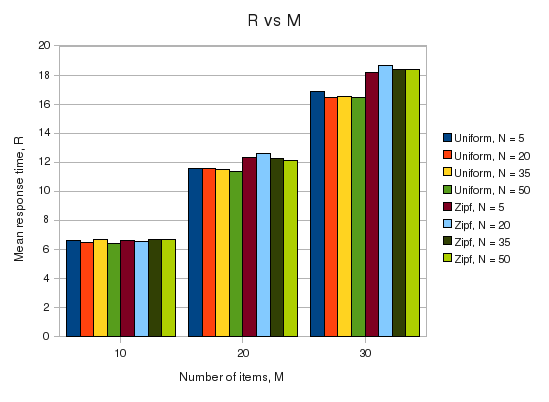
\includegraphics[height=10cm]{R_vs_M.png}
\end{center}
\end{table}

This chart clearly illustrates the effect that varying $M$ (the number of
f-items) has on the mean response time $R$.  Larger values of $M$ produce larger
values of $R$ regardless of $N$ or the distribution used for $p_m$.  This can be
very easily explained.

Each f-item is transmitted in a cycle, with an average transmit time of 1.
Since our simulation runs for a finite length of time, we can clearly see that
if we have more f-items, each one will be transmitted less times, and thus less
frequently.  Of course, if each item is transmitted less frequently, then each
individual request will be serviced slower, and thus that will increase the mean
response time $R$, as we see in the chart above.

The slight difference between zipf and uniform distributions comes from the fact
that large $M$ values means more items, which means more requests are for items
further away from 6.  This slightly increases the mean response time.


\newpage
\begin{table}[htp!]
\subsection{Effect of $N$ on $R_m$}
\begin{center}
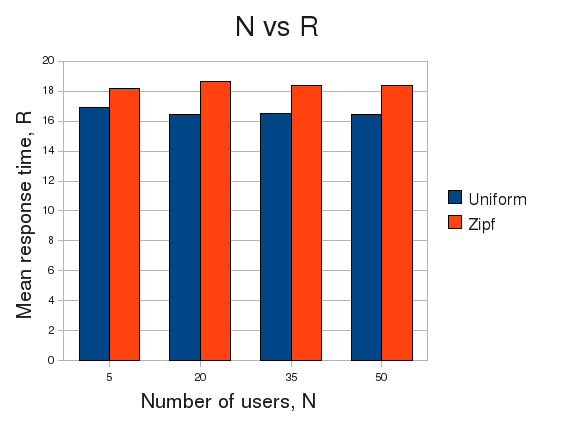
\includegraphics[height=10cm]{R_vs_N.png}
\end{center}
\end{table}

This chart shows how varying number of users, $N$, affects the mean response
time $R$.  For this chart, the value $M = 30$ was chosen arbitrarily since we
saw in the previous section that varying $N$ has the same effect on $R$
independent of $M$.

It is quite obvious to see from the chart that varying the number of users has
little influence on $R$.  This can also be easily explained.  The model works in
way such that user's requests are stored on their workstation, and the server
uses a broadcast method to serve up the frequently requested items.  In
broadcast mode, the server only broadcasts the items and any number of users can
listen to the broadcast without impacting the transmit time.  From there, it is
logical to conclude that increasing the number of users will only increase the
number of requests, and not how often each request is services.  Since the
distribution remains the same, the mean will be unaffected as we see in the
chart.

\section{Part e) Finding an Optimal $G$}
\begin{table}[htp!]
\subsection{Data}
\begin{center}
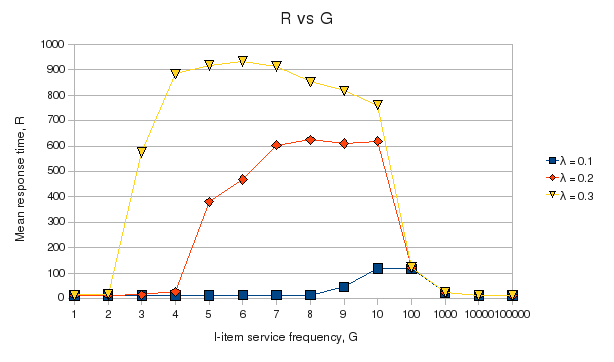
\includegraphics[height=10cm]{R_vs_G.png}
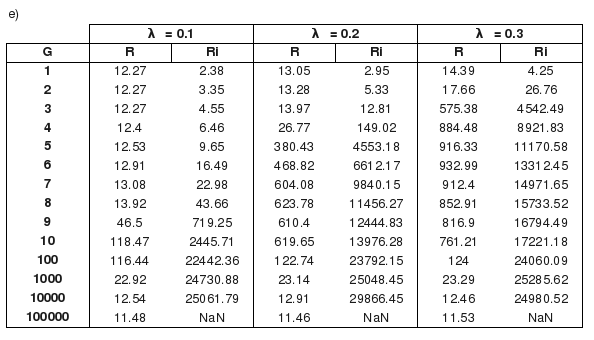
\includegraphics[height=8cm]{part_e.png}
\end{center}
\end{table}

\subsection{Analysis}
The chart above shows the relationship between the frequency of servicing
i-items, $G$, and the mean response time, $R$, for various values of $\lambda$.
Note that $R$ values for larger $G$ are also provided at an exponential scale.
That data used to create the chart is also provided above.

From the chart we see that for the most part, the smaller $R$ is, the smaller
$G$ is.  This would lead us to believe that $G=1$ is the optimal choice.
However, we must first consider a couple other special cases.

First, we notice that for $G > L$, we get an even smaller $R$.  In this case, it
is obvious that not a single i-request is serviced, and thus only f-requests are
handled.  Although strictly speaking this gives us a lower $R$, we should not
have to completely stop sending i-items, and so this case is discarded.
Similarily, for very large $G$ (see $G=10000$), only a handful of i-items are
serviced.  This causes little impact on the mean response time, however we see
that the i-item response times are way too large and these cases should also be
discarded.

We could also consider the case in which $G=0$.  In this case, only i-items are
serviced and f-requests are completely ignored.  This situation is so against
our common sense that I did not evaluate $R$ values for such a situation, and it
to is ignored.

Ignoring these impractical cases, we are left with $G=1$ being the ideal value
to minimize mean response time.

\end{document}
